95. \begin{figure}[ht!]
\center{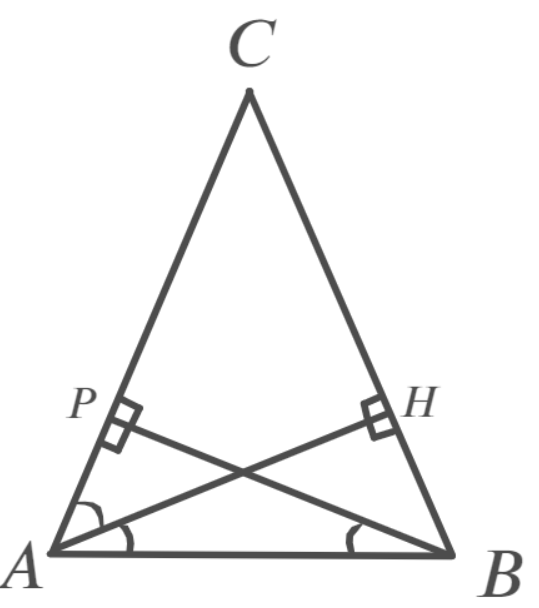
\includegraphics[scale=0.35]{g95.png}}
\end{figure}\\
$\left.\begin{array}{l}BP=AH,\\
AB\text{ --- общая.} \end{array}\right\}\Rightarrow \Delta BPA=\Delta AHB\text{ по катету и гипотенузе}\Rightarrow \angle HAB=\angle ABP=\angle CAH.$ Тогда из треугольника $APB$ имеем $\angle CAH=90^\circ:3=30^\circ,$ тогда $\angle C=\angle B=\angle A=60^\circ.$\\
